\begin{figure*}%[!htbp]
\begin{center}
\thinmuskip=-2mu
\thickmuskip=-2mu
\nulldelimiterspace=-1pt
\scriptspace=0pt
\begin{minipage}{\textwidth}%
\begin{minipage}{0.5\textwidth}%
\begin{subfigure}[b]{\columnwidth}%
  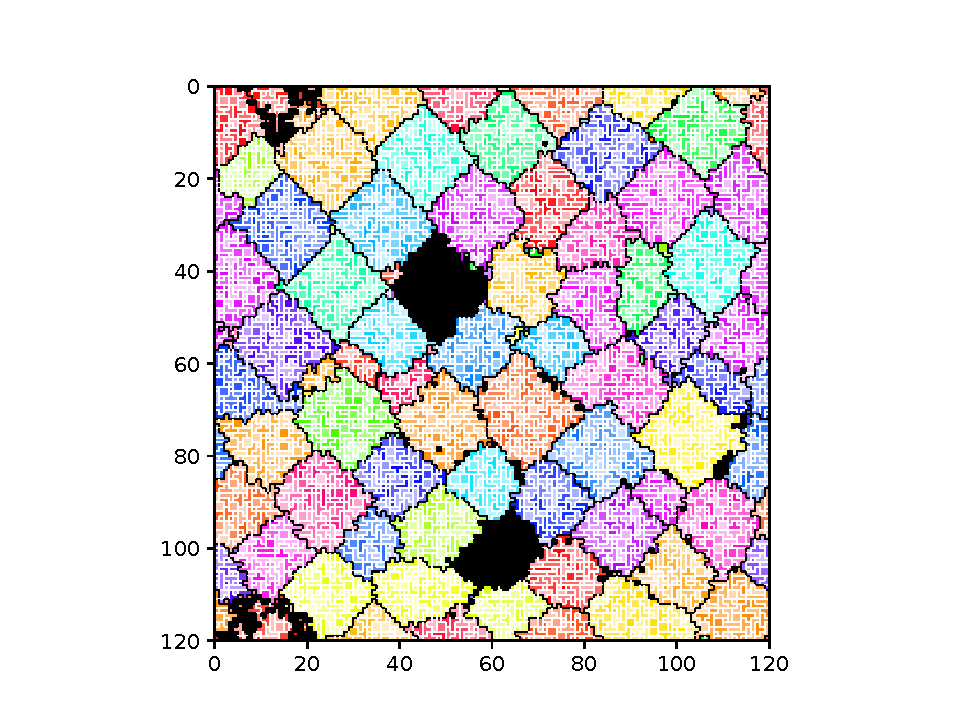
\includegraphics[width=\columnwidth,trim={2.5cm 0.5cm 2.5cm 1cm},clip]{img/ChannelMap_1044_update20000000}
  \caption{Mean $P_{c} = 0.03$, $P_1 = 0.75$, $P_2 = 0.23$; cell gen. 29920}
  \label{fig:ChannelMap_1044}
\end{subfigure}%
\end{minipage}%
\begin{minipage}{0.5\textwidth}%
\begin{subfigure}[b]{\columnwidth}%
  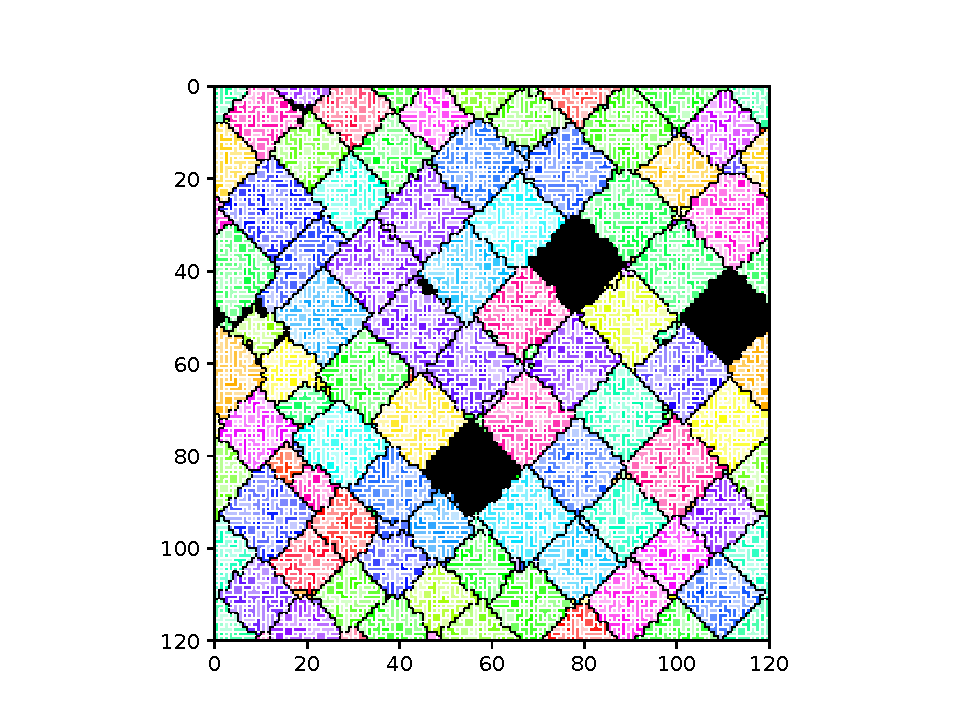
\includegraphics[width=\columnwidth,trim={2.5cm 0.5cm 2.5cm 1cm},clip]{img/ChannelMap_1016_update20000000}
  \caption{Mean $P_{c} = 0.03$, $P_1 = 0.51$, $P_2 = 0.49$; cell gen. 33852}
  \label{fig:ChannelMap_1016}
\end{subfigure}
\end{minipage}%
\end{minipage}

\begin{minipage}{\textwidth}%
\begin{minipage}{0.5\textwidth}%
\begin{subfigure}[b]{\columnwidth}%
  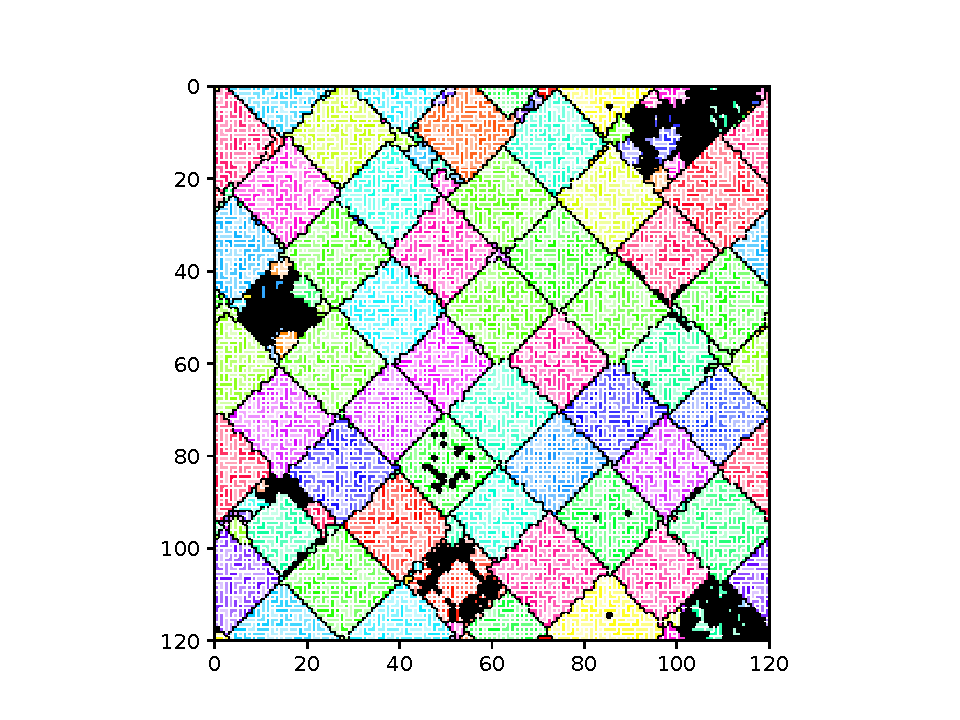
\includegraphics[width=\columnwidth,trim={2.5cm 0.5cm 2.5cm 1cm},clip]{img/ChannelMap_1007_update20000000}
  \caption{Mean $P_{c} = 0.08$, $P_1 = 0.01$, $P_2 = 0.90$; cell gen. 47507}
  \label{fig:ChannelMap_1007}
\end{subfigure}
\end{minipage}%
\begin{minipage}{0.5\textwidth}%
\caption{
End state of same-channel signaling networks in replicates where resource was exclusively allocated to first-level channel pools (\ref{fig:ChannelMap_1044}), was split evenly between first- and second-level channel pools (\ref{fig:ChannelMap_1016}), and was primarily allocated to second-level channel pools (\ref{fig:ChannelMap_1007}).
Level-one channels are coded by color saturation and level-two channels are coded by color hue.
A single cell-like organism occupies each grid tile except for black tiles, which are empty.
Level-one same-channel groups appear as uniformly-colored clumps, bounded by a white border.
Level-two same-channel groups appear as same-hue amalgamations of level-one groups, bounded by a black border.
}
\label{fig:outcome_grids}
\end{minipage}%
\end{minipage}
\end{center}
\end{figure*}
